\documentclass[10pt,twocolumn]{article}

% ------------------ PAQUETES ------------------
\usepackage[spanish]{babel}
\usepackage[utf8]{inputenc}
\usepackage[T1]{fontenc}
\usepackage{geometry}
\usepackage{graphicx}
\usepackage{amsmath, amssymb}
\usepackage{siunitx}
\usepackage{authblk}
\usepackage{abstract}
\usepackage{caption}
\usepackage{titlesec}
\usepackage{multicol}
\usepackage{hyperref}
\usepackage{currfile}
\usepackage{float}

\geometry{margin=1.8cm}

% ------------------ FORMATO DE SECCIONES ------------------
\titleformat{\section}{\large\bfseries}{\thesection}{1em}{}
\titleformat{\subsection}{\normalsize\bfseries}{\thesubsection}{1em}{}

% ------------------ TÍTULO ------------------
\title{\textbf{Aproximación manual a la fotometría de apertura}\\Trabajo sobre el cúmulo abierto Messier 41\\Tercera parte: Introducción al machine learning}


% ------------------ AUTORES ------------------
\author[1]{Bruno Abello Laurent}

\affil[1]{Universidad de Los Andes, Departamento de Física, Colombia}

% Correos (puedes modificar)
\renewcommand\Authands{, }
\date{}

\begin{document}

\twocolumn[
\maketitle
\begin{center}
\small
\textit{Correo institucional:} \href{mailto:{b.abello@uniandes.edu.co}}{b.abello@uniandes.edu.co} \\
\textit{Repositorio de GitHub: } \href{https://github.com/Brunelleschk1/Personal-projects/tree/main/Proyectos\%20de\%20Astronom\%C3\%ADa/Laboratorio\%203}{Repositorio del laboratorio}
\end{center}

\begin{abstract}
\noindent
Este informe es el segundo en una lista semanal cuyo objetivo es el acercamiento del autor a los métodos computacionales que se utilizan a menudo en el dominio de la astrofísica 
para definir la pertenencia de una estrella a un cúmulo abierto. El presente se enfoca en la determinación de pertenencia mediante un método de machine learning llamado HDBSCAN.
La idea de este método es aprovechar parámetros como la densidad de puntos en un VPD para definir un cluster. Puesto que trabajos pasados se han centrado en métodos previos 
al machine learning, hoy se realiza una comparación entre el método de machine learning y el anterior método utilizado. 
\end{abstract}

\noindent\textbf{Palabras clave:} Messier 41, HDBSCAN, Vector Point Diagram, Color Magnitude Diagram. 
\vspace{0.5cm}
]

% ------------------ CONTENIDO ------------------

\section{Introducción}

La semana anterior se terminó el informe con la esperanza de encontrar el cúmulo gracias a la primera
implementación de Machine Learning. El presente informe tiene como objetivo comparar este método
al método utilizado la semana pasada, de manera a concluir sobre la necesidad y la utilidad de cada método
y su potencia. Lo cierto es que, si bien llevamos haciendo una revisión histórica de los métodos implementados, 
esta vez vamos a dar un pequeño salto, ya que HDBSCAN no es el primero que se implementó en el estudio de 
cúmulos estelares. El primero fue la versión no jerarquizada del segundo, por lo que el segundo es más poderoso
que el primero, y por ende se puede ver que la necesidad de trabajar con el primero no es necesario ni muy útil:
el salto de potencia entre métodos varia relativamente poco comparado con el salto que hemos tenido entre 
las semanas anteriores, y como tal el uso de HDBSCAN solo trae ventajas y un mejor entendimiento de la 
capacidad de los métodos de machine learning. 

La diferencia grande entre los métodos de la semana anterior y esta implica que necesariamente tenemos que
utilizar un nuevo conjunto de datos, ya que HDBSCAN funciona con diferencias de densidades entre puntos, 
por lo cual un set de poca densidad como el utilizado la semana anterior no funcionará correctamente 
cuando se aplice el algoritmo. Este informe es entonces la comparación de los dos métodos con un 
único conjunto de datos, uno con muchas más estrellas, que abarca una mayor porción del cielo. Por ende, 
no se ha de preocupar el lector por tener que caminar entre el informe de la semana anterior y este, 
ya que este cada uno es consistente con su tema y no requiere de otros para entenderse, aunque sea 
una entrada en una serie de eventos sucesivos. 

\subsection{Objetivos}

Los objetivos que tenemos, en términos simples, son los siguientes:
\begin{itemize}
    \item Implementar un método de Machine Learning para la detección de cúmulos estelares. 
    \item Comparar este método a un método clásico de optimización de parámetros.
    \item Empezar a familiarizarnos con la manera en la que se realizan los códigos de Machine Learning
    \item Acercarnos a la forma en la que se obtienen resultados con métodos de machine learning 
    \item Entender las limitaciones del Machine Learning y la necesidad de análisis humano
\end{itemize}


\section{Procedimiento}

El procedimiento que se siguió esta semana tuvo principios muy distintos a los de las semanas anteriores. 
Primeramente, esta vez no se empezó un código de cero, sino que se empezó a trabajar con un notebook 
ya estructurado y completo, que contenía la manera de implementar DBSCAN y HDBSCAN para un conjunto de datos.
Posteriormente, se descargó un nuevo conjunto de datos, más grande, de GAIA DR3. Con esto logrado, 
se estructuró el notebook para que respondiera a nuestras necesidades: la creación de una serie de VPDs
y de CMDs que nos muestren qué encuentra HDBSCAN en términos de simple pertenencia y en términos de la
silueta de los miembros encontrados por el algoritmo. Además, se importó al nuevo ambiente de trabajo
el código de la semana anterior y se modificó para que pudiera trabajar correctamente en su nuevo lugar. 
Se guardaron los resultados de ambos códigos para su comparación lado a lado, tanto número de miembros
como diagramas de interés. 

\section{Problemas presentados y soluciones aplicadas}

\begin{enumerate}
  \item  El primer problema encontrado fue a la hora de empezar a trabajar con un notebook y no con un archivo 
  de python clásico. No conocía cómo asignar el ambiente de trabajo adecuado para JuPyter, por lo que tuve 
  varios problemas para poder siquiera correr el código. 
  \item En segundo lugar, el archivo era supremamente extenso, y la parte de HDBSCAN se encontraba al fondo del mismo, 
  por lo que abrir el documento y llegar a la parte interesante era demorado, especialmente cuando se tenía que correr
  todo por primera vez. La solución, obviamente, fue eliminar toda la parte de DBSCAN y todo el texto explicativo por 
  fuera del código, ya que, si bien es interesante, no nos sirve para tener un código claro y directo. 
  \item El siguiente problema surgió con la presentación de resultados: no conseguía generar unas gráficas 
  que me gustaran, ya fuera por color o por contenido. Al final, tras prueba y error de hiperparámetros y de 
  correcciones de gráficas, obtuve un resultado compacto y agradable, que contiene exactamente lo que uno esperaría
  en un estudio del funcionamiento del machine learning.
  \item Los demás problemas fueron, sobretodo, con el tiempo para trabajar en este proyecto. Debido a que no estoy
  familiarizado con el método, ni con otros conceptos aledaños, encontrar el tiempo de trabajar correctamente en esto
  por encima del estudio de parciales fue complicado, razón por la cual este informe llega más tarde que los demás.
  Los problemas en este caso fueron sobretodo aprender a poner en marcha el método y aprender a presentar el método
  correctamente, y no tanto de implementación del mismo. Esto no es muy sorprendente: las funciones de python 
  realizan todo el trabajo por debajo, ya no estamos metiendo la mano directamente en lo que ocurre, contrariamente
  a la optimización de parámetros que fue, en gran parte, trabajo de los laboratoristas
\end{enumerate}

\section{Resultados}

Los resultados, esta vez, son bastante escuetos: se pueden mostrar en una imagen(Fig: ~ \ref{resultadosCompletos})(aunque mostrarlo en varias vaya a ser necesario para la correcta comprensión
del contenido.) Vemos dos resultados distintos: los CMDs y los VPDs. Los VPDs muestran el ruido y ambos clusters encontrados con su silueta. Aunque parezca que el ruido tiene todos los miembros
en su interior, lo cierto es que tiene dos huecos en lugar de ambos clusters. Lo mismo sucede con los CMDs, donde pareciera que el ruido ocupa todos los miembros. 
La realidad se ve cuando se observan los demás diagramas, donde el gris representa el fondo, y los colores representan los cúmulos. 

\begin{figure}[H]
    \centering
    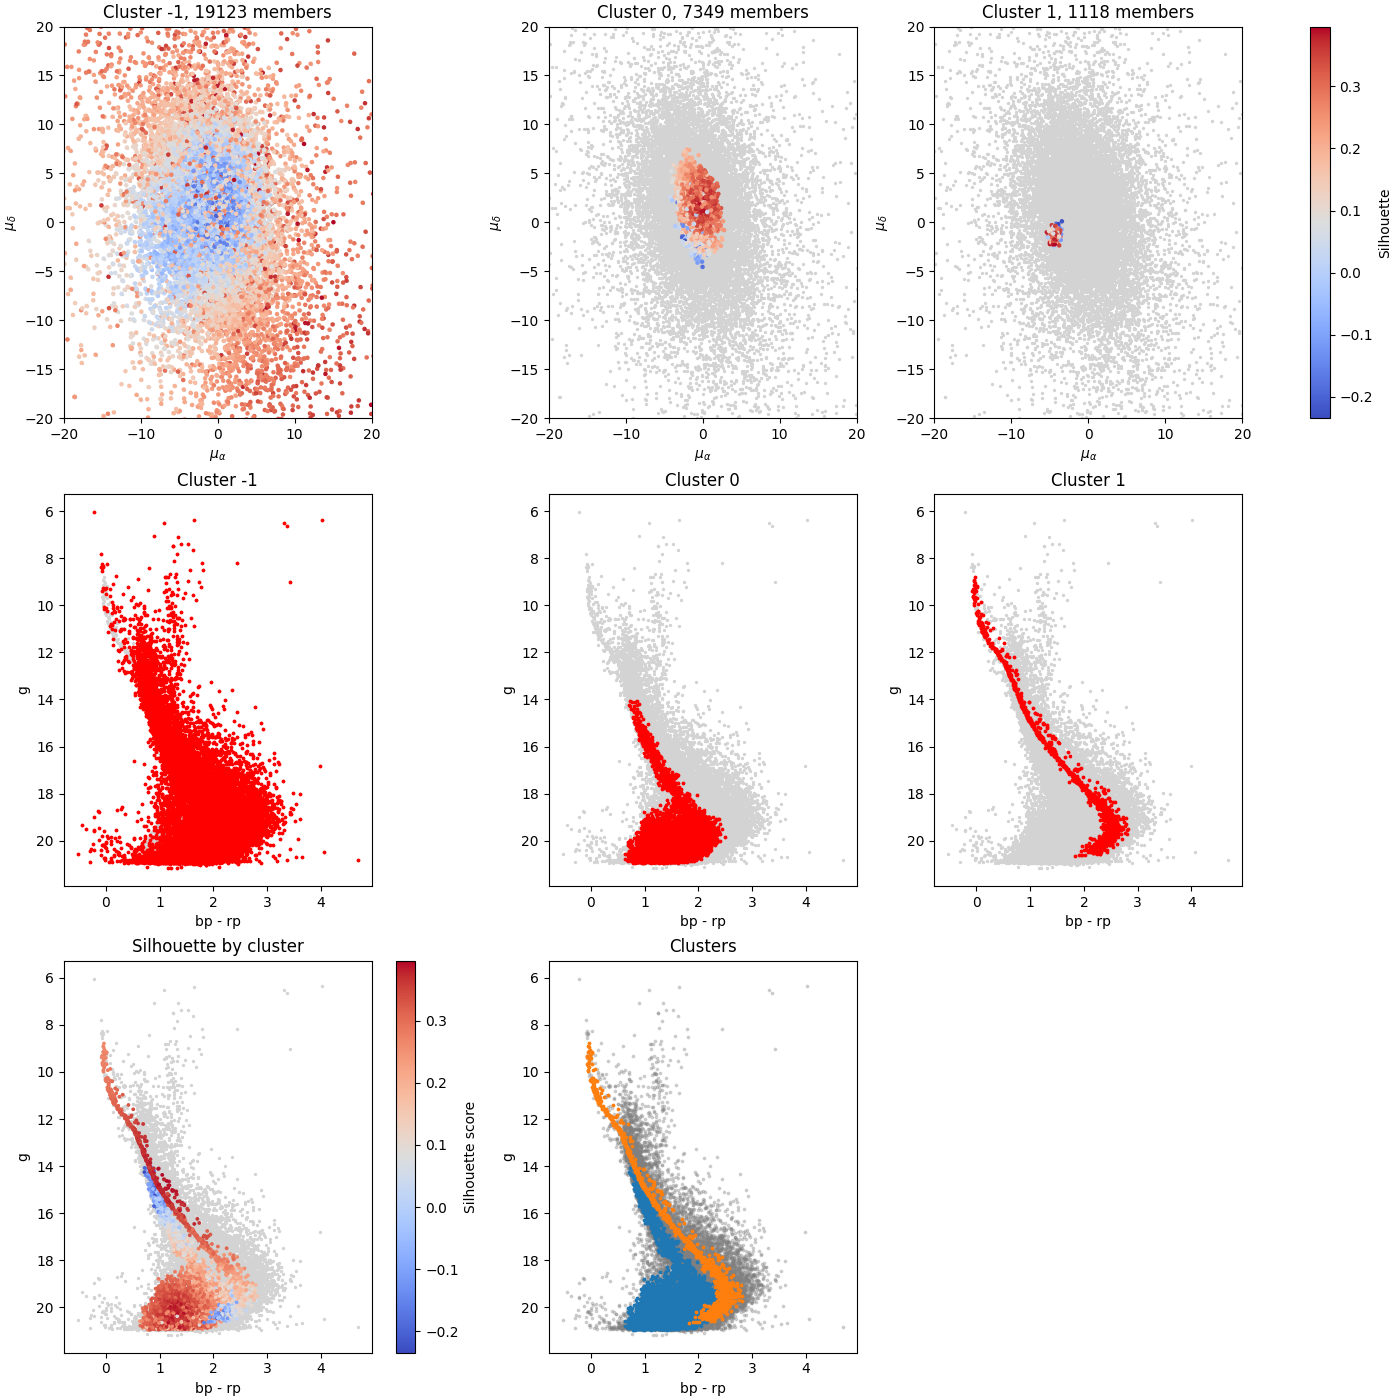
\includegraphics[width=0.8\linewidth]{../Resultados_completos.png}
    \caption{Compilación de los CMDs obtenidos con el estudio de los datos mediante HDBSCAN. El cluster Messier 41 es,
    se espera, el cluster 1 tal y como lo marca el método.}
    \label{resultadosCompletos}
\end{figure}

El cúmulo 0, de más de 7000 miembros, no nos interesa mucho, ya que normalmente no debería haber uno. De este resultado solo se puede concluir que, si bien HDBSCAN es un excelente
método para encontrar clusters, el hecho de que encuentre un cluster no significa que sea uno real, solo que, para los parámetros que se estipularon, esa densidad de objetos 
se parece a un cúmulo. por ende son resultados que, si bien vamos a mostrar en los gráficos comparativos, solo lo utilizaremos para mostrar, como se dijo en la introducción, 
la necesidad de análisis humano a pesar de la potencia de los computadores. 

Lo realmente interesante para nostros de HDBSCAN se encuentra en las imágenes (Fig: ~\ref{VPDHDB}, \ref{CMDHDB}, \ref{CMDSILHD}). Vemos una secuencia principal definida, 
diferenciada entre miembros singulares y binarios, mientras que los miembros más alejados de la secuencia principal tienen un valor de silueta bajo, poniendo en duda su 
pertenencia al cúmulo M41. Nótese que aquí ya se filtraron valores de silueta bajos(inferiores a 0.1), llevando el número de miembros a 968 miembros. Sin hacer esto, 
se encuentran 1181 miembros. En general, ignorando las particularidades de M41, estos resultados apuntan a un cúmulo bien constituido y con miembros cuya pertenencia 
está bien definida. 

\begin{figure}[H]
    \centering
    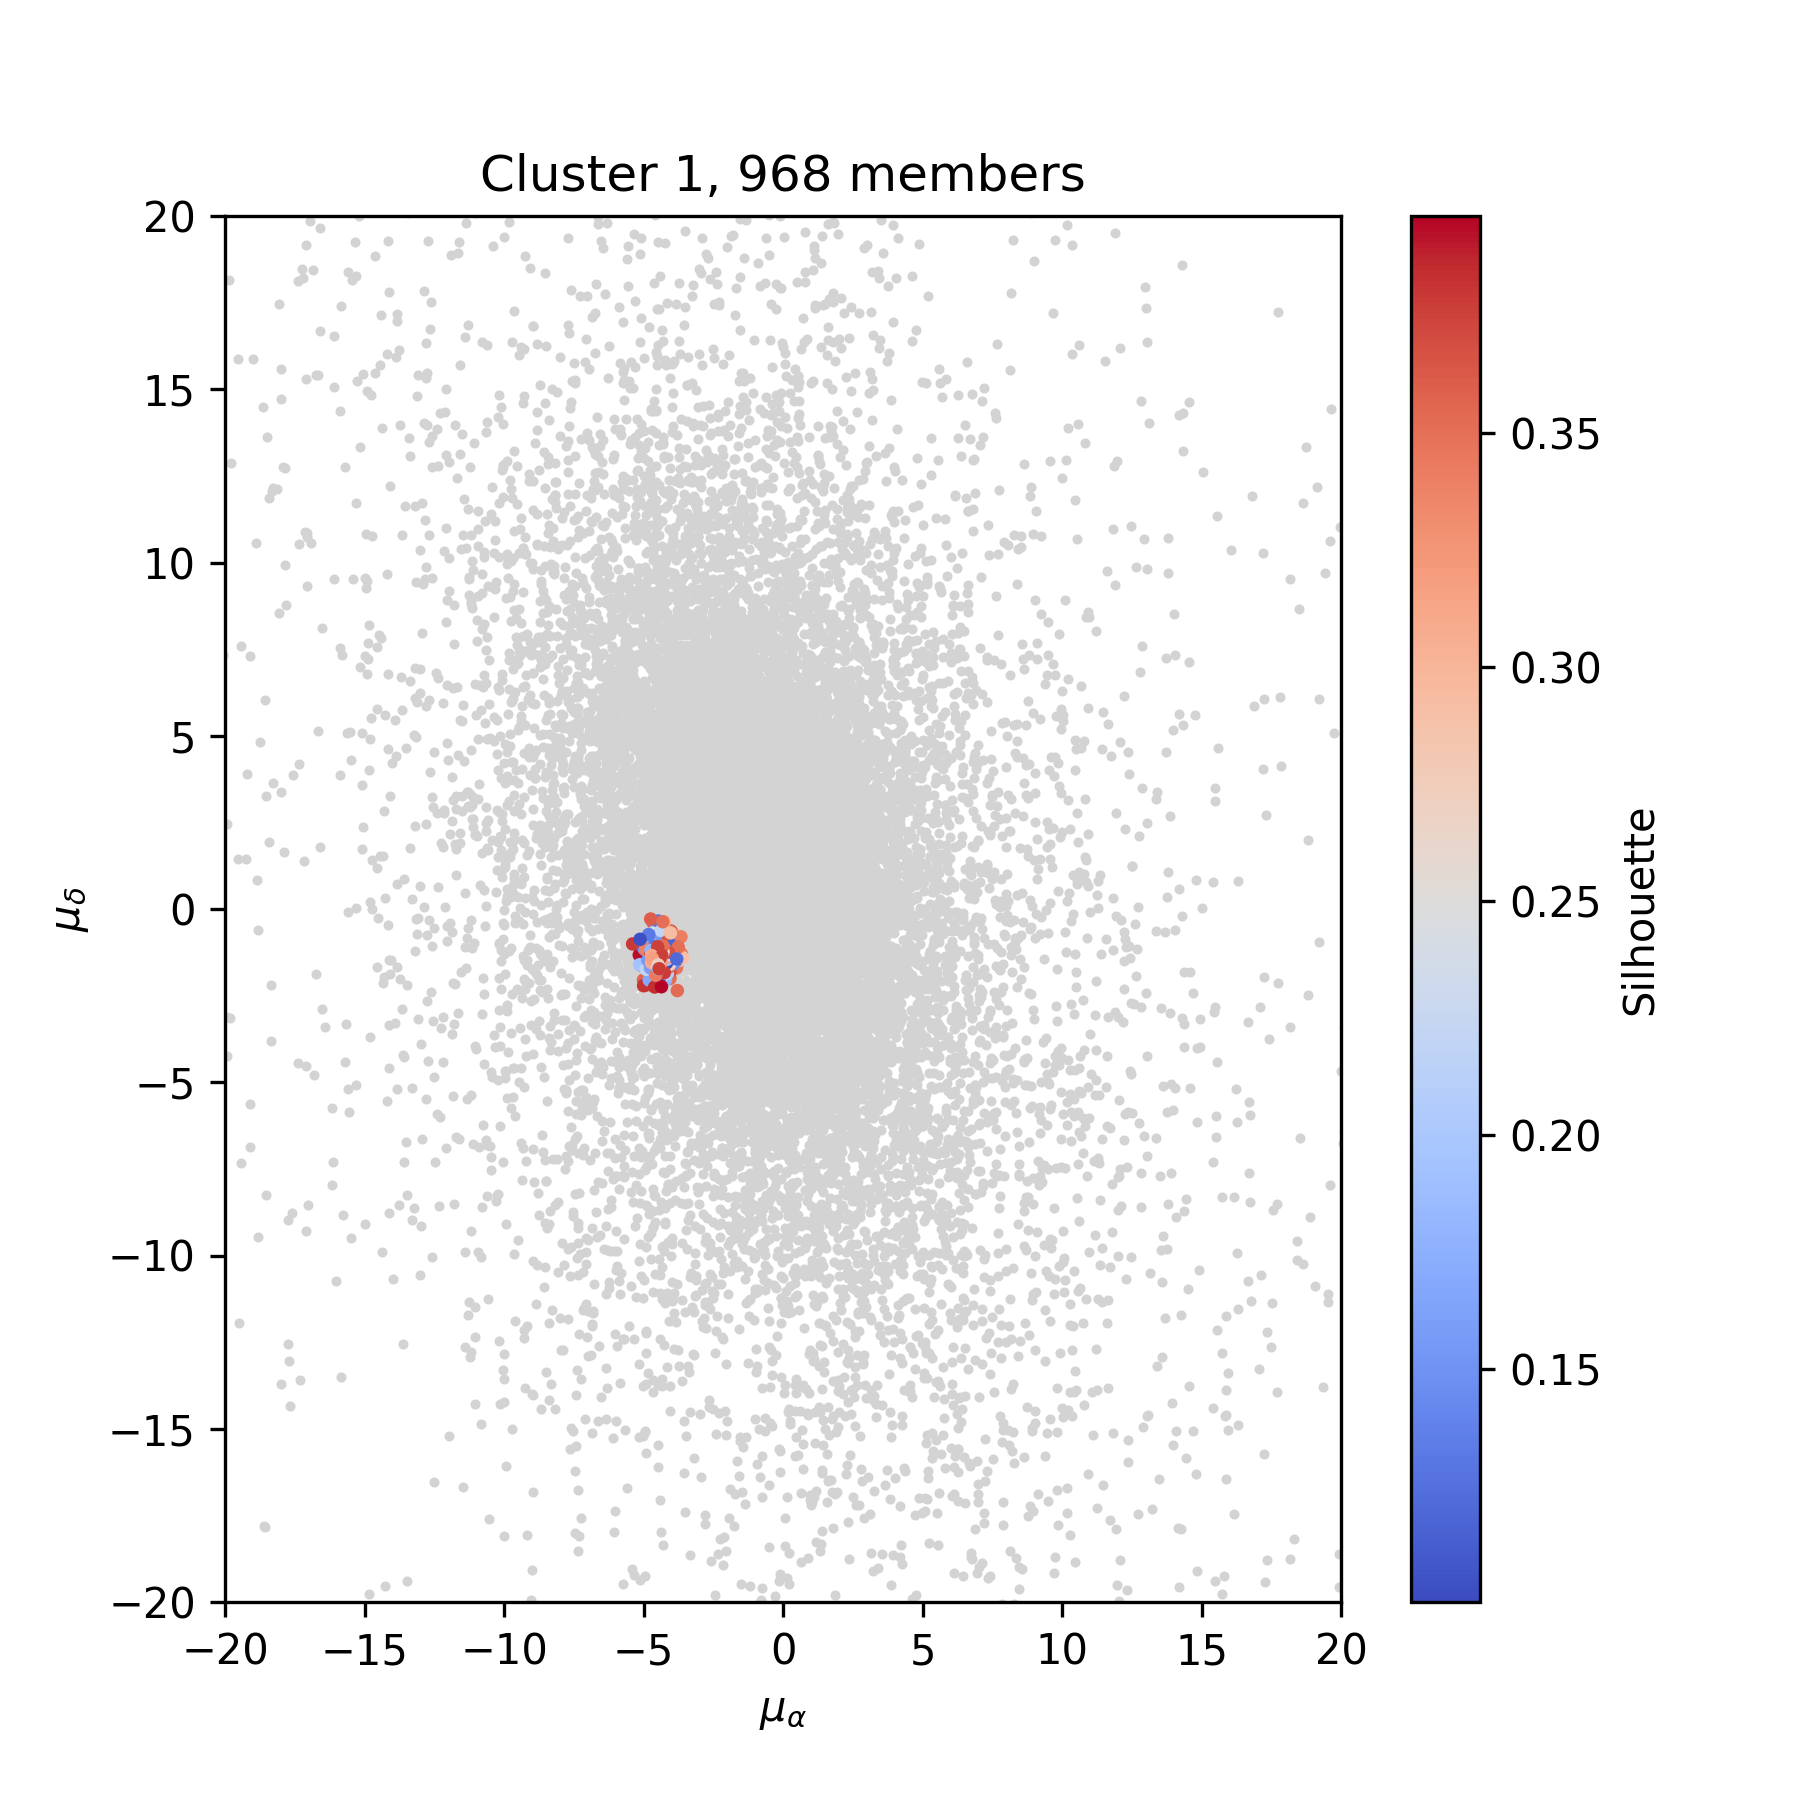
\includegraphics[width=0.8\linewidth]{../paneles/VPD_cluster_1.png}
    \caption{VPD mostrando el cúmulo M41 por silueta. Se ve una buena densidad de estrellas con buena silueta, y unos pocos con una silueta más baja.}
    \label{VPDHDB}
\end{figure}

\begin{figure}[H]
    \centering
    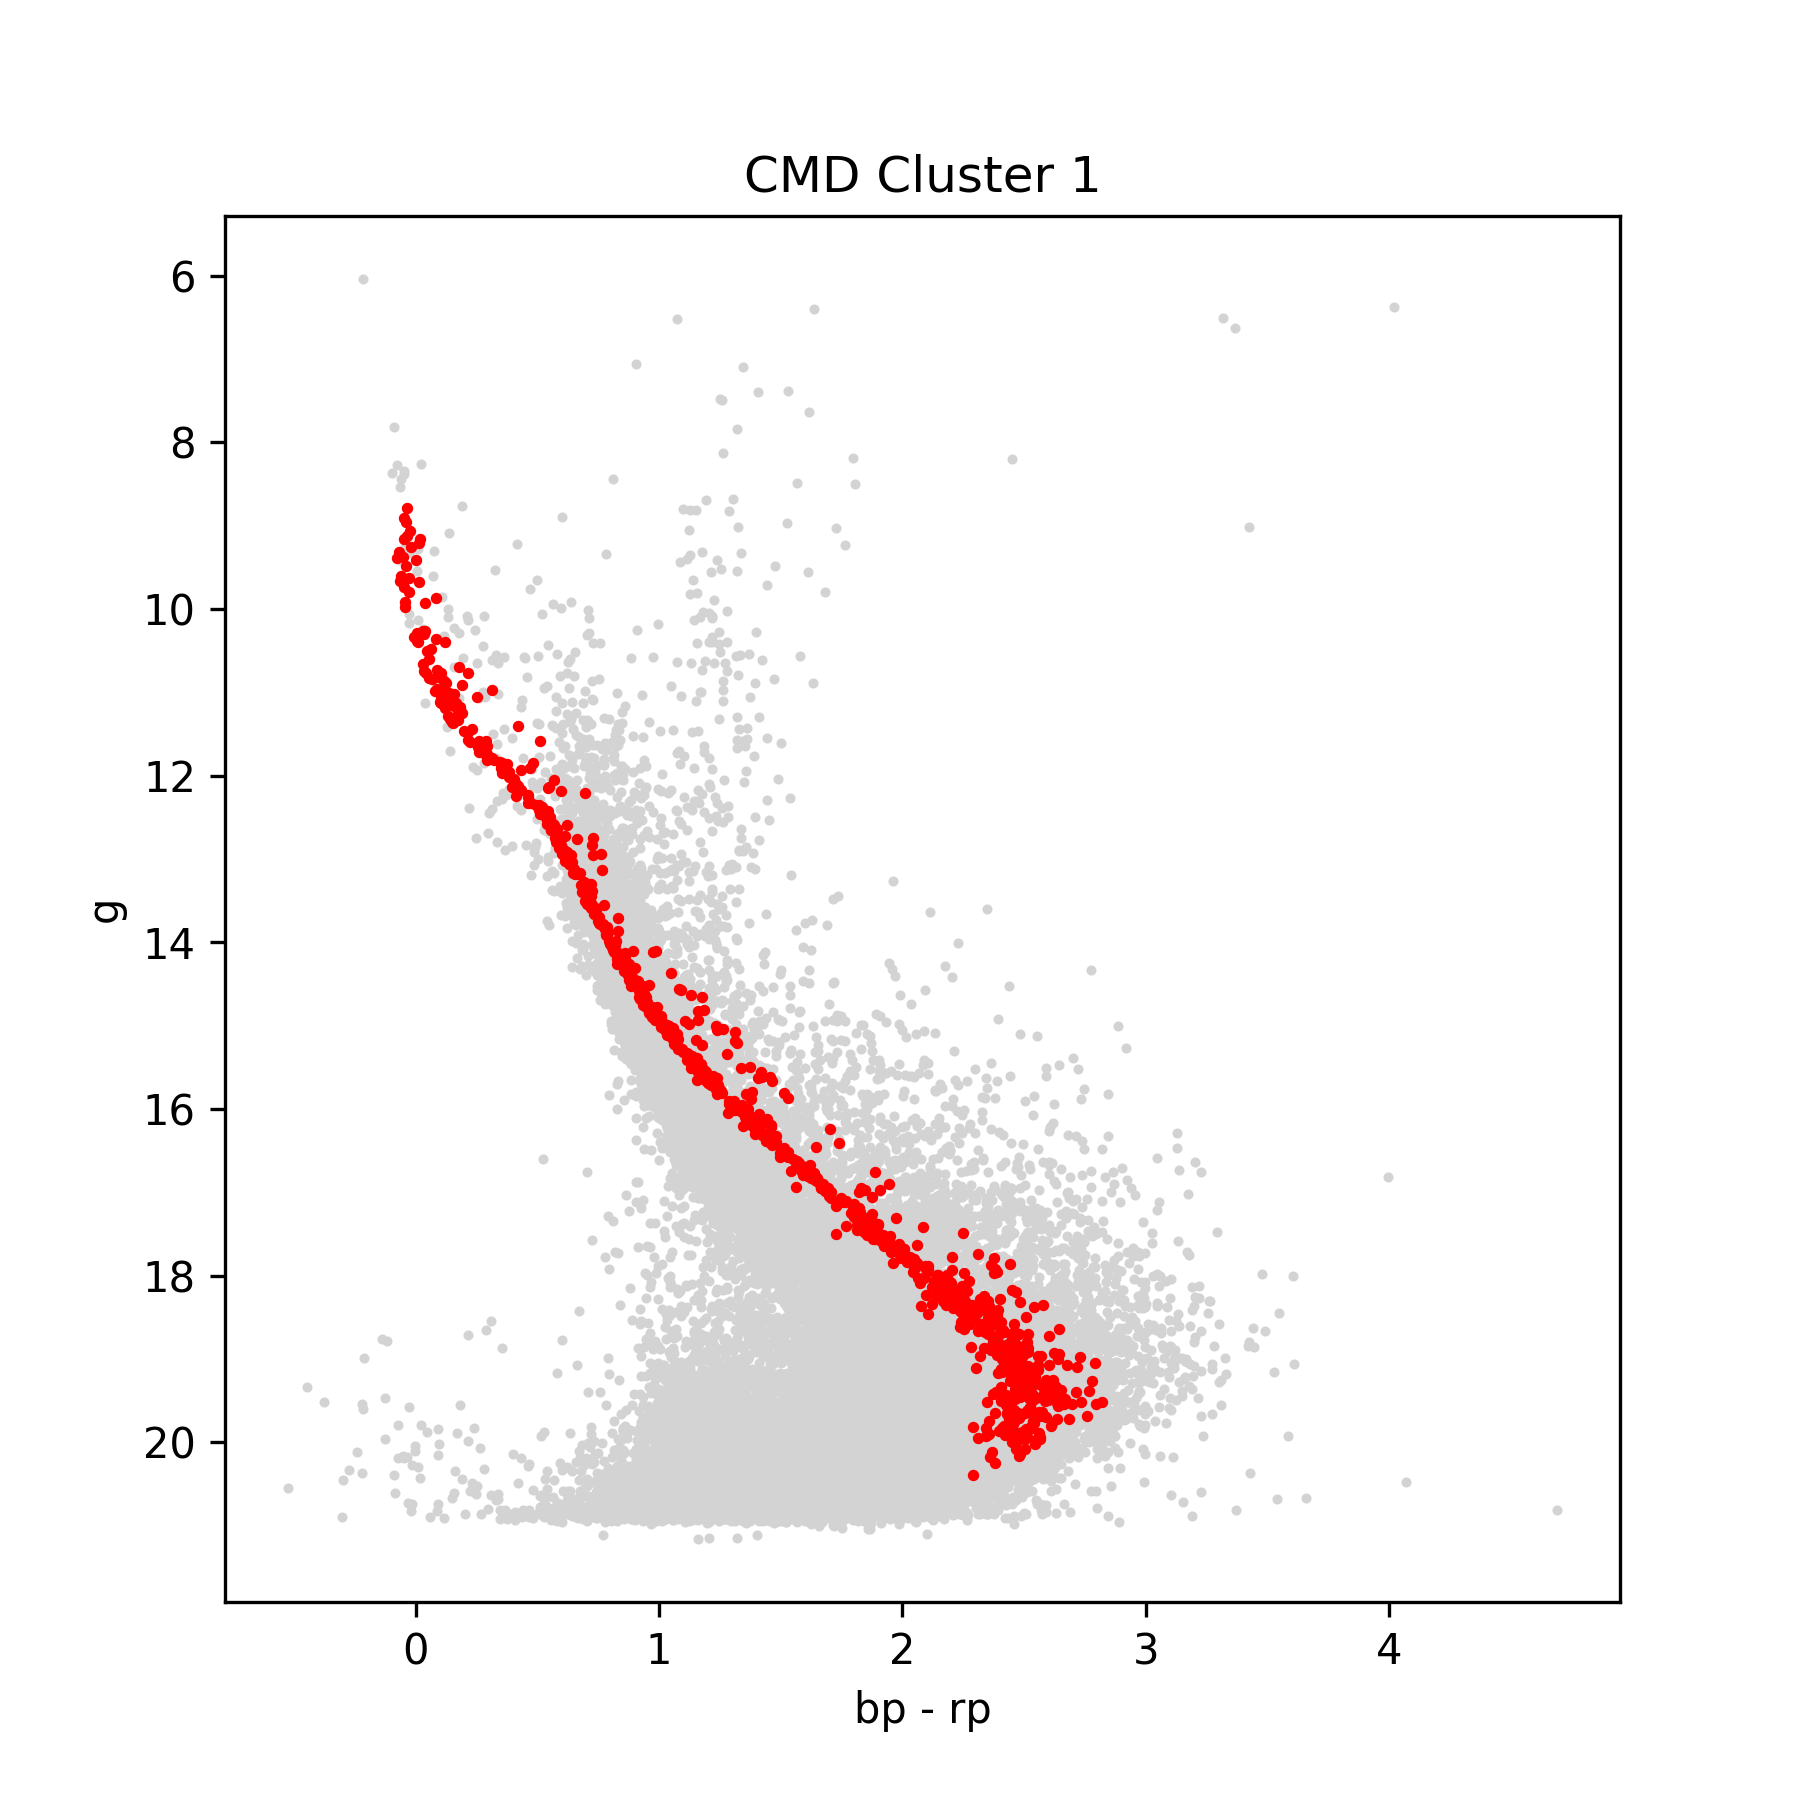
\includegraphics[width=0.8\linewidth]{../paneles/CMD_cluster_1.png}
    \caption{CMD mostrando la comparación entre el fondo y el cúmulo M41. Se ve una secuencia principal concreta, con algunas estrellas binarias,
    por lo que se puede decir que es un resultado correcto dentro de lo esperado de un CMD. Este CMD es complementario a (Fig: ~ \ref{CMDSILHD}), donde se 
    ven ambos clusters graficados con su valor de silueta.}
    \label{CMDHDB}
\end{figure}

Por otro lado, tenemos los resultados del código clásico, utilizado la semana anterior en el análisis. Los resultados de esto son visibles en las imágenes 
(Fig: ~ \ref{CMD}, \ref{ProbPert}). Se ve, en el CMD, una secuencia principal bien definida para miembros con probabilidad mayor a 0.9 de pertenecer, así 
como una buena distribución de probabilidades de pertenencia en el histograma. Este método encuentra 886 estrellas con probabilidad superior a 0.9 de 
pertenecer al cúmulo, pero más de 1200 estrellas según el ajuste de parámetros. Los VPDs encontrados muestran una buena densidad de estrellas,
de manera similar al informe anterior. Nótese que el único cambio que se hizo en el código fue el nombre del archivo que se iba a leer. 
El círculo marcando pertenencia en el VPD se dejó intacto(Fig:~\ref{VPDOpt}), lo confirma que, debido a que buscamos en la misma región del cielo, estamos 
estudiando el mismo cúmulo que la semana pasada. 

Vemos resultados similares, aunque para el método clásico haya que ser bastante estricto con la probabilidad de pertenencia para encontrar casi que el 
mismo CMD que en el caso de HDBSCAN. La pregunta que queda, además de que vemos que el machine learning hace, entre comillas, un mejor trabajo que los métodos 
clásicos debido a no necesitar parámetros iniciales y a encontrar resultados fácilmente analizables con poco esfuerzo, es si estos resultados concuerdan con
los de la semana anterior y con los que se espera en la literatura. 

\begin{figure}[H]
    \centering
    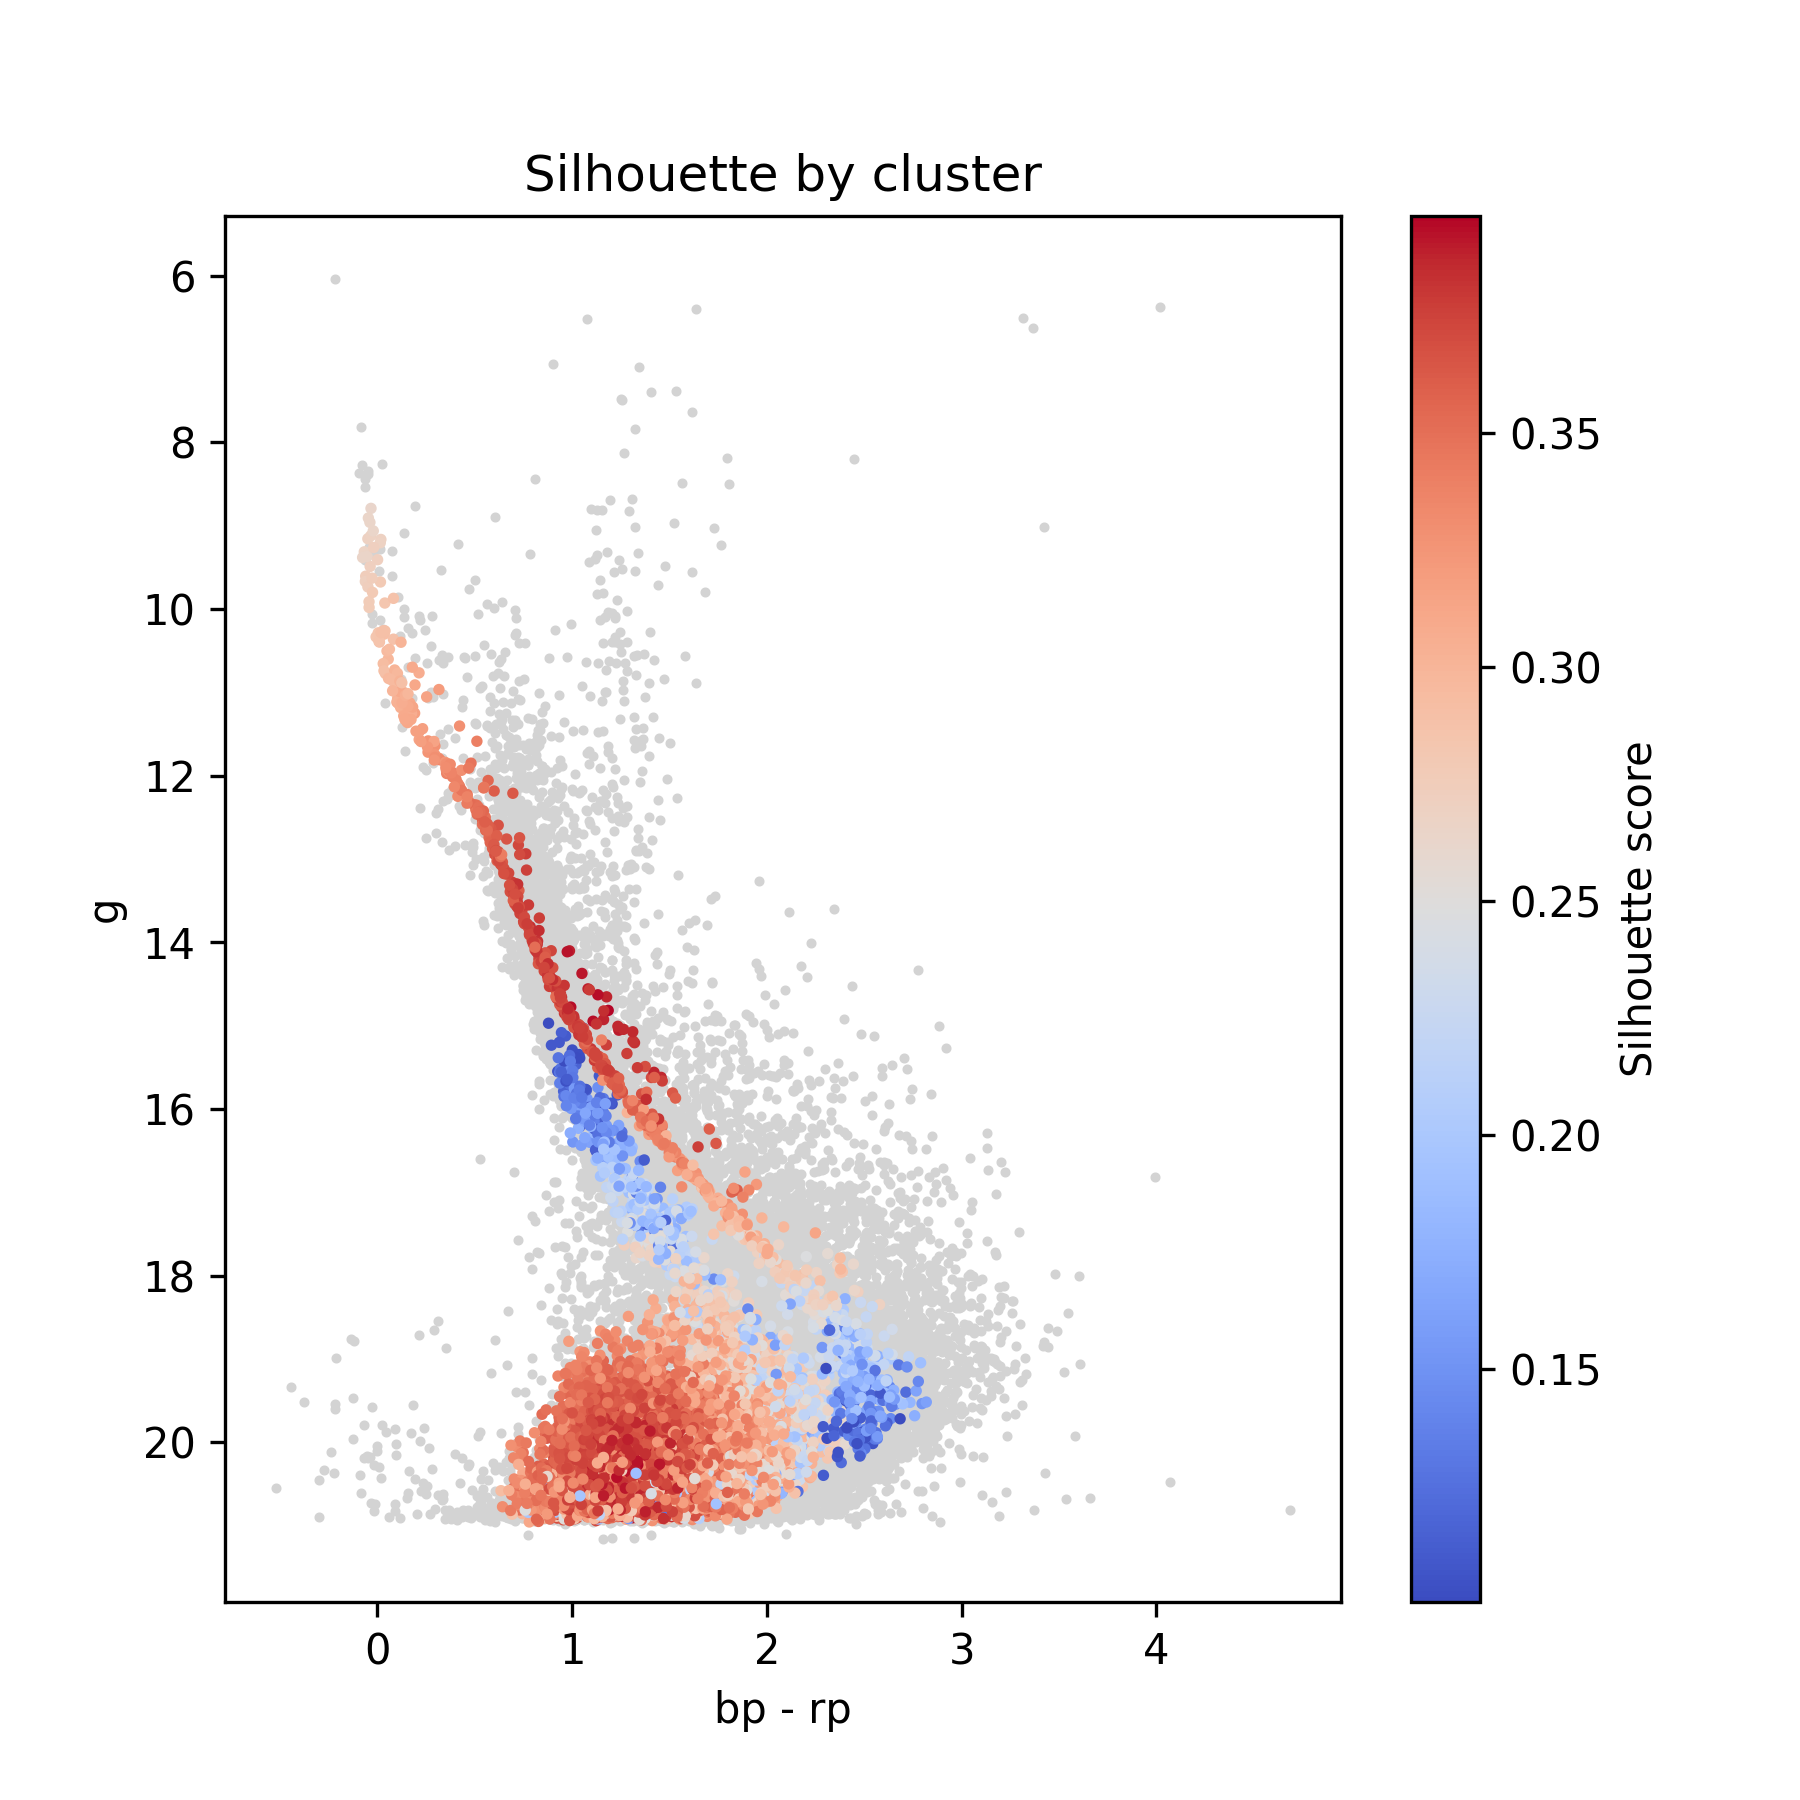
\includegraphics[width=0.8\linewidth]{../paneles/CMD_silhouette.png}
    \caption{CMD mostrando ambos clusters con su valor de silueta por miembro. Para el cluster de interés, identificado mediante el CMD (Fig: ~ \ref{CMDHDB}), 
    se ven unos miembros con silueta alta alrededor de la secuencia principal. Los de silueta más baja se encuentran antes de que empieze la secuencia principal.
    Esto es algo esperable, ya que para un cúmulo abierto se esperan miembros únicamente en la secuencia principal, sean binarios o singulares.}
    \label{CMDSILHD}
\end{figure}

Los resultados del número de miembros pertenecientes a M41 ha aumentado a lo largo de los años: De 300 miembros en 2013(\cite{Kharchenko2013}), pasando por 
714 en 2018 (\cite{Sun2019}), 625 y 660 en 2020(\cite{CantatGaudin2020}) y 2022(\cite{Tarricq2022}), para llegar a 849 miembros en 2023(\cite{vanGroeningen2023}). 
Desde entonces, hemos recibido la tercera entrega de datos de GAIA, por lo que tenemos muchos más miembros, y por ende el resultado obtenido de entre 
800 y 1000 estrellas suena bastante razonable. Podríamos pensar que, comparados con los poco más de 500 miembros encontrados la semana anterior, 
este resultado nuevo está sobreestimando el número de miembros que existen en el cúmulo. Sin embargo, ya que estos nuevos resultados se acercan más 
a los de la literatura, y debido a la cantidad mayor de datos descargados en esta ocasión, se puede aceptar con facilidad que Messier 41 tiene, 
de verdad, toda esta cantidad de miembros. Hay que tener cuidado, sin embargo, ya que se supone que no deberían haber miembros por fuera de 
la secuencia principal, tanto por debajo como por arriba, por lo que podríamos decir que la cantidad de miembros encontrada es levemente mayor
a la real. 

\begin{figure}[H]
    \centering
    
\includegraphics[width=0.8\linewidth]{../CMDPintadoErr.png}
    \caption{CMD mostrando el resultado obtenido por el método de optimización de parámetros. Se ve una buena pertenencia a la secuencia principal, con un par de 
    miembros perdidos hacia la parte superior, todo para una probabilidad de 0.9 o más. }
    \label{CMD}
\end{figure}

\begin{figure}[H]
    \centering
    
\includegraphics[width=0.8\linewidth]{../ProbPertU.png}
    \caption{Histograma de probabilidad de pertenencia al cúmulo de interés, en escala logarítmica. La forma en U esperada se nota a pesar de la escala. }
    \label{ProbPert}
\end{figure}

\begin{figure}[H]
    \centering
    
\includegraphics[width=0.8\linewidth]{../VPDColoreado.png}
    \caption{VPD del método de optimización de parámetros. Se observa que la región estudiada se encuentra en el mismo lugar que en el método de Machine Learning,
    y se observa una buena densidad de puntos.}
    \label{VPDOpt}
\end{figure}

\section{Conclusiones}

Para concluir este tercer informe sobre nuestro estudio a Messier 41, se ha de decir que nuestro estudio ha llegado muy lejos gracias a la aplicación 
de métodos computacionales cada vez más modernos y potentes. Ahora, estamos en el dominio del Machine Learning, y los resultados del método nos han 
mostrado lo poderosa que es esta manera de resolver problemas de pertenencia. Vimos no solo cómo se hace sencillo resolver el problema, sino también
que hay nuevos métodos que nos permiten definir aún mejor la pertenencia a un cúmulo gracias a los métodos de Machine Learning. 

Asimismo, vimos que el machine learning tiene sus limitaciones a la hora de entender lo que es y no es un cúmulo de verdad, a pesar de la densidad de 
puntos que se le muestre, y que por ende la intervención humana en el análisis sigue siendo necesaria. De este modo, el problema de entender 
qué pertenece y qué no al cúmulo se vuelve un problema de qué consideramos cúmulo y qué no, y qué consideramos que es correcto dentro del método
y qué no, como lo evidencian el recorte por valor de silueta o por probabilidad de pertenencia. 

\section*{Comentarios al margen}

Haciendo este informe se tuvieron muchos problemas de tiempo, debido probablemente a un estado de cansancio del autor. 
Lo cierto es que, gracias a una semana de descanso, el autor puede recuperarse y completar este estudio. 
El siguiente informe, si bien seguirá siendo con HDBSCAN, ya no será sobre Messier 41. Esta serie de tres informes 
llega entonces a su fin, y fue una buena manera de acercarnos a cómo se hace la astrofísica moderna. 

\bibliographystyle{apalike}
\bibliography{refs}
\end{document}